%% Versão final IEEE
\documentclass[a4paper]{IEEEtran}

% Versão com uma coluna
%\documentclass[journal,12pt,onecolumn,]{IEEEtran}
%\usepackage[a4paper, marginparwidth=1in]{geometry}

% Versão Rascunho com uma coluna
%\documentclass[journal,12pt,onecolumn,draftclsnofoot,]{IEEEtran}
%\usepackage[a4paper, marginparwidth=1in]{geometry}

%



\usepackage[utf8]{inputenc}
\usepackage{epstopdf}
%\usepackage[spanish]{babel}
\usepackage[cmex10]{amsmath,nccmath}
%\interdisplaylinepenalty=2500
\usepackage{amsfonts}
\usepackage{amssymb}
\usepackage{graphicx}
\usepackage{verbatim}
\usepackage{array}
%\usepackage{multirow}
\usepackage{dcolumn}
\usepackage{color}
\usepackage[noadjust]{cite}
\usepackage{url}
\usepackage{balance}
\usepackage[usenames,dvipsnames]{xcolor}
\usepackage{accents}
\usepackage{blindtext}
%\usepackage{soul}
\usepackage[normalem]{ulem}
\usepackage{pgf,tikz}
\usetikzlibrary{arrows}
%\DeclareGraphicsExtensions{.eps} % eu que comentei
%\AppendGraphicsExtensions{.pdf} % eu que comentei


% % % Adicionados por mim
%\usepackage[colorinlistoftodos]{todonotes}
\usepackage[colorinlistoftodos,prependcaption,textsize=small]{todonotes}
\usepackage{xargs} 

\newcommandx{\todoi}[2][1=]{\todo[linecolor=Plum,backgroundcolor=Plum!25,bordercolor=Plum,#1,inline]{#2}}
%\newcommand{\todop}[1]{\todo[textsize=tiny]{#1}}
%%%%



\DeclareMathOperator*{\Max}{max}
\DeclareMathOperator*{\Min}{min}
\DeclareMathOperator*{\argmin}{arg\,min}
\DeclareMathOperator*{\Maximize}{Maximize}

\begin{document}
\title{Scenario generation for nongaussian time series via Quantile Regression
}

\author{Marcelo~Ruas~%,~\IEEEmembership{Student Member,~IEEE,}
	and Alexandre~Street,~\IEEEmembership{Member,~IEEE}	
	
	
	%\thanks{This work was partially supported by UTE Parna\'iba Gera\c{c}\~ao de Energia S.A. through R\&D project ANEEL PD-7625-0001/2013.}
	%\thanks{Bruno Fanzeres, Arthur Brigatto and Alexandre Street are with the Electrical Engineering Department, Pontifical Catholic University of Rio de Janeiro (PUC-Rio), Rio de Janeiro, RJ, Brazil (e-mail: \mbox{bsantos@ele.puc-rio.br}; \mbox{street@ele.puc-rio.br}).}
	%\thanks{L. A. Barroso are with PSR Consulting, Rio de Janeiro, RJ, Brazil (e-mail: \mbox{luiz@psr-inc.com}).}
}

\maketitle


%\begin{abstract}
%	\blindtext
%\end{abstract}

\begin{IEEEkeywords}
	Quantile Regression, Model Identification, Non-gaussian time series model
\end{IEEEkeywords}


\listoftodos


% ===== Sec. I - Introduction ===== %

\section{Introduction}

% % % Talk about renewable energy and its variability

Renewable energy power is a hot topic in the recent years. It is a much cleaner way of producing energy than by using other sources such as coal and gas, and with less hazard potential than nuclear power plants. The installed capacity of renewable plants has been increasing in a fast pace and projections point that wind power alone will account to 18\% of global power by 2050  \cite{IntEnerAgency}.
In spite of being a welcoming technology, it brings new challenges for power system planners, operators, and agents. It is important to have good forecasts of either high and low quantiles
 the complex behavior of wind is very difficult to model and predict.  \todo{é importante prever bem quantis altos e baixos p analise de risco - fica prejudicada pela dificuldade de previsao destes quantis }
Having better prediction models can help the planner to make better and less risky decisions, increasing the attractiveness of renewable energy to the energy system. 
In this work we will investigate how to model dynamics of renewable energy time series in both short and long terms.

% % % Critics about point forecasts and gaussian models (ARIMA-GARCH). Compare GAS and nonparametric models. 

Conventional statistics are often focused on estimating the conditional mean of a given random variable.
\todoi{Falar sobre modelos de previsão usando modelos tradicionais para energia renovável}
 This is not very useful when dealing with renewable energy, as the variability and the notion of risk is extremely important for planning. Our attention is, then, turned to probabilistic forecasting models. Among these, there are many possibilities. \cite{zhang_review_2014} reviews the commonly used methodologies for this task, separating them in parametric and nonparametric classes. Main characteristics of \textbf{parametric models} are (i) assuming a distribution shape and (ii) low computational costs. ARIMA-GARCH, for example, model the renewable series by assuming the distribution \textit{a priori}. On the other hand, \textbf{nonparametric models} (i) don't require a distribution to be specified, (ii) needs mode data to produce a good approximation and (iii) have a higher computational cost. Popular methods are Quantile Regression, Kernel Density Estimation,  Artificial Intelligence or a mix of them.


% % % Talk about nonparametric models and how to use quantile regression to estimate the whole distribution

A common finding is that wind and solar time series don't have a Gaussian behavior. Furthermore, we can't point any distribution that fits on the data undoubtedly. For this reason, we choose to use a nonparametric approach, more specifically the Quantile Regression (QR), as defined in \cite{koenker2005quantile}.
As we are working with time series, we rely on the results of \cite{koenker_quantile_2006}, which defines the quantile autoregression, extending the application of QR on cases where the covariates are lagged values of $y_t$. 
QR is a powerful tool for measuring quantile others than the median. By estimating many quantiles on a thin grid of probabilities, one can have as many points as desired of the estimated conditional distribution function.

However, when estimating a distribution function, as each quantile is estimated independently, the monotonicity of the distribution function may be violated. This issue is a known as crossing-quantiles. To get around it we propose to either add a constraint on the optimization model or make a transformation as in \cite{chernozhukov_quantile_2010}, which can be estimated independently.

Using QR as in \cite{koenker2005quantile} is not a novelty when predicting the conditional distribution of wind power time series, as is already done in \cite{moller_time-adaptive_2008,nielsen2006,bremnes_probabilistic_2004,wan_direct_2017}.
In this article, we combine QR with regularization techniques. On the Mixed Integer Linear Programming (MILP) approach, we use the best subset selection, which \cite{bertsimas_best_2015} does for minimizing the quadratic error and the $\ell_1$ penalization as in \cite{belloni_l1-penalized_2009} or \cite{ciuperca_adaptive_2016} (the AdaLasso variant, where each coefficient may have a different weight on the objective function to ensure oracle properties).
On the advantages of QR we highlight the fact that it is a direct way of finding a given quantile directly and it is data driven, so it doesn't depend on distribution assumptions. 

%% Review of quantile regression for wind and solar

\todoi{Review of quantile regression for wind and solar - procurar mais referências?}

The approach by \cite{gallego2016line} is to use QR with a nonparametric methodology. The authors add a penalty term based on the Reproducing Kernel Hilbert Space, which allows a nonlinear relationship between the explanatory variables and the output. This paper also develops an on-line learning technique, where the model is easily updated after a new observation.

In \cite{wan_direct_2017}, QR is used with a special type of Neural Network (NN) with one hidden layer, called extreme learning machine. In this setup, each quantile is a different linear combination of the features of the hidden layer. 


 



%%%% Contributions
The objective of this paper is to propose a new methodology to address nonparametric time-series focused on renewable energy. In our analysis, we develop both nonlinear and linear models for QR. The main contributions are:
\begin{itemize}
	\item A nonparametric methodology to model the conditional distribution of a given time series.
	
	\item On the linear case, we propose a parsimonious methodology that selects the global optimal solution with a given number of 
	
	\item Regularization techniques applied to an ensemble of quantile regressions to estimate the conditional distribution
	
	\item 
	
\end{itemize}

We propose a new combination of methods to predict the $k$-step ahead conditional distribution. By using MILP, we achieve a solution which is optimal for the given objective. In order to improve the quality of predictions and interpretability, we incorporate a joint regularization by specifying the existence of groups among the probabilities $\alpha$. We could not find any other work in the literature that interpreted different quantiles as models depending on one another. 
The objective of this paper is to propose and test different techniques of predicting the conditional distribution based on QR. 


% OBJETIVOS:
Um modelo para séries tmeporais autoregressivo e nao parametrico e baseado na função quantilica. No caso autoregressivo, uma metodologia de estimação com seleção parcimoniosa otima global é proposta e possibilita o controle dos números de grupos de regressores diferentes dentro do modelo para diferentes quantis. Para o modelo não paramétrico
Modelo data driven, empirico


% Next sessions paragraph

The remaining of the paper is organized as follows. In section II, we present both the linear parametric and the nonlinear QR based time series models. In section III, we discuss the estimation procedures for them. The regularization strategies are also presented on this section. Finally, in section IV, a case study using real data from both solar and wind power is presented in order to ...
Section V will conclude this article.



%2) Quantile Regression based time series model
%	A. Linear parametric explanatory model
%	B. General non-linear nonparametric model
%
%3) Estimation procedures
%	A. Linear model with optimal variable selection / regularization
%	B. Nonlinear model
%	
%4) Case study
%	A. Long term wind power generation
%	B. Short term wind (solar?) generation
%
%5) Conclusion





% % Seguir a estrutura paragrafo papaer henrique

%1) Motivacao para minimizar o risco da WPG
%2) Fala sobre a pesquisa em WPG utilizando ARMA e SARIMA com distribuição gaussiana 

% % Colocar em especifico os objetivos e detalhar os papers anteriores, destacando o que o nosso tem e nenhum outro atingiu ate entao

% procurar os objetivos que já discutimos.









% % % % % % % % % % % % % % % % % % %

%As opposed to the conventional work of doing a model to forecast the
%conditional mean, our work focus on finding a distribution for $y_{t}$
%on each $t$. 
%
%We find a time series model, based on quantile autoregression (as
%in Koenker 2005).
%
%As we are interested in the whole distribution of $\hat{y}_{t+k|t}$,
%we estimate a phin grid of quantiles in $0<\alpha_{1}<\alpha_{2}<\dots<\alpha_{|A|}<1$,
%such that the distribution can be well approximated.
%
%As a Quantile Autoregression model, we are interested in selecting
%the best subset of variables do model the time series. 
%
%As we are trying to model the whole $k$-step ahead distribution,
%we estimate many quantiles. We didn't find any previous work where
%a given $\alpha$-quantile model influenced another model.
%
%In all works found, each quantile is estimated separately. 
%
%Regularization can be done by introducing a penalty on the $\ell_1$-norm of the coefficients. The work by \cite{belloni_l1-penalized_2009} defines proprieties and convergence analysis. The AdaLasso variant, where each coefficient may have a different weight on the objective function to ensure oracle proprieties, is developed on \cite{ciuperca_adaptive_2016}.

% ===== Sec. II - Quantile Regression ===== %
%
\section{Quantile Regression based time series model} \label{sec:qr1}

Let the $\alpha$-conditional quantile function of $Y$ for a given value $x$ of the $d$-dimensional random variable $X$, i.e., $Q_{Y|X}:[0,1] \times \mathbb{R}^d \rightarrow \mathbb{R}$, can be defined as %(in short, from now on, $Q_{Y|X}(\cdot, \cdot)$)
\begin{equation}
Q_{Y|X}(\alpha,x) = F_{Y|X}^{-1}(\alpha,x) = \inf\{y: F_{Y|X}(y,x) \geq \alpha\}.
\label{eq:quantile-function}
\end{equation}
Let a dataset be composed from $\{y_t,x_t \}_{t \in T}$ and let $\rho$ be the check function 
\begin{equation}\label{eq:check-function}
\rho_{\alpha}(x)=\begin{cases}
\alpha x & \text{if }x\geq0\\
(1-\alpha)x & \text{if }x<0
\end{cases}.
\end{equation}
The sample quantile function for a given probability $\alpha$ is then based on a finite number of observations and is the solution to minimizing the loss function $L(\cdot)$:
\begin{IEEEeqnarray}{C}
\hat{Q}_{Y|X}(\alpha,\cdot)\quad\in\quad  \underset{q\in\mathcal{Q}}{\text{arg min}}\, L_\alpha(q) = \sum_{t\in T}\rho_{\alpha}(y_{t}-q(x_t)),\label{eq:optim-lqr1} 
\end{IEEEeqnarray}
The $\alpha$-quantile function $q_\alpha$ belongs to a function space $\mathcal{Q}$. We might have different assumptions for space $\mathcal{Q}$, depending on the type of function we want to find for $q$. A few properties, however, must be achieved by our choice of space, such as being continuous and having limited first derivative. In this paper, we consider the case where $\mathcal{Q}$ is a linear function's space.

The quantile function is approximated by a sequence of $|J|$ (where $J$ is an index set) quantiles $q_{\alpha_1} \leq q_{\alpha_2} \leq \dots \leq q_{\alpha_{|J|}}$. 
We also define the closely related set $A = \{ \alpha_j \mid j \in J \}$, whose elements all must range on $[0,1]$, for they are probability values such that $0 < \alpha_1 < \alpha_2 < \dots < \alpha_{|J|} < 1$. The sequence $\{ \alpha_j \}_{j \in J}$ provides a finite discretization of the interval $[0,1]$. 

Problem (\ref{eq:optim-lqr1}) can be rewritten as a Linear Programming problem as in (\ref{eq:linear-opt-1})-(\ref{eq:linear-opt-ult}), thus being able to use a modern solver to fit our model. Variables $\varepsilon^+_t$ and $\varepsilon^-_t$ represent the quantities $|y-q(\cdot)|^+$ and $|y-q(\cdot)|^-$, respectively. This new formulation estimates all quantiles at the same time, and we denote $q$ as $q_\alpha$ to differentiate it from each $\alpha$.
{\tiny }\begin{IEEEeqnarray}{lr}
\min_{\beta_{0j},\beta_j,\varepsilon_{tj}^{+}, \varepsilon_{tj}^{-}} \, \sum_{j \in J} \sum_{t \in T}\left(\alpha_j \varepsilon_{t j}^{+}+(1-\alpha_j)\varepsilon_{t j}^{-}\right)
 \span \label{eq:linear-opt-1}\\
\mbox{subject to} \span \nonumber \\
\varepsilon_{t j}^{+}-\varepsilon_{t j}^{-}=y_{t} - \beta_{0j} - \beta_{j}^T x_{t}, & \forall t \in T, \forall j \in J, \\
\varepsilon_{tj}^+,\varepsilon_{tj}^- \geq 0, & \forall t \in T,\forall j \in J,\\ 
\beta_{0j} + \beta_{j}^T x_{t} \leq \beta_{0,j+1} + \beta_{j+1}^T x_{t}, \span \nonumber \\
\span \label{eq:linear-opt-ult} \forall t \in T, \forall j \in J_{(-1)},
\end{IEEEeqnarray}
To estimate a conditional distribution based on quantile values, all quantiles $\{q_\alpha \}_{\alpha \in A}$ are estimated simultaneously. With the addition of constraint (\ref{eq:linear-opt-ult}), we assure the monotonicity of the quantile function, solving the issue of crossing-quantiles.
The output is the sequence $\{ q_\alpha \}_{\alpha \in A}$, which is fully defined by the optimum values $\beta^*_{0\alpha}$ and $\beta^*_\alpha$, for each $\alpha$.

We apply QR to estimate the conditional distribution $\hat{Q}_{Y_{t+h}|X_{t+h},Y_t, Y_{t-1}, \dots} (\alpha,\cdot)$ for a $h$-step ahead forecast of time serie $\{y_t\}$, where $X_{t+h}$ is a vector of exogenous variables at the time we want to forecast. Once the conditional distribution is estimated, we are able to simulate and generate scenarios. In the next session, regularization techniques are presented, in order to choose parsimoniously which variables will be input for $\hat{Q}$.

%Let $A$ be a set containing a sequence of probabilities  $\alpha_i$ such that $0 < \alpha_1 < \alpha_2 < \dots < \alpha_Q < 1$. This set represents a finite discretization of the interval $[0,1]$.
%One of our goals with quantile regression is to estimate a quantile function $\hat{Q}_{Y|X}$ of a given real valued random variable $X$ from a sequence of quantiles $q_{\alpha_1}(x_t) \leq q_{\alpha_2}(x_t) \leq \dots \leq q_{\alpha_{|A|}}(x_t)$, with $0 < \alpha_1 < \alpha_2 < \dots < \alpha_{|A|} < 1$, for any given $t$.
%The process of fitting $\hat{Q}_{Y|X}$ is by mapping every $\alpha_i$ with its estimated quantile $\hat{q}_{\alpha_i}(x_t)$.
%The denser the grid of values in $A$, better is the approximation of $Q_{Y|X}$.
%Thus, the distribution found for $Y$ is nonparametric, as no previous assumptions are made about its shape, and its form is fully recovered by the data we have.
%
%The crossing quantile is a common issue when estimating a set of quantiles \cite{chernozhukov_quantile_2010}. Two a solution may be 
%
%
%A typical problem, however, arises when working with quantile regression. When quantiles are estimated independently, it is possible to find $q_{\alpha}(x_t) > q_{\alpha'}(x_t)$, for a given $t$, when $\alpha_1 < \alpha_2$. An example can be seen on Figure \ref{fig:crossing-quantiles}, where quantiles $\alpha = 0.95$ and $\alpha = 0.9$ cross. This problem, called \textit{crossing quantiles}, can be prevented by estimating all quantiles with a single minimization problem.
%
%
%
%As opposed to traditional parametric models where one has to assume the error distribution on the model
%\begin{equation}
%y_t = h(F_t) + \varepsilon_t,
%\end{equation}
%as we choose the nonparametric methodology we are released from this step. A distribution for $\varepsilon_t$ is defined within the estimation procedure. The predictive distribution is derived from the individual quantiles
%\begin{equation}
%\hat q^\alpha_{t+k|k} = \hat y_{t+k|t} + \hat F^\varepsilon_{t,k}(\alpha).
%\end{equation}
%% % coisas aqui % %
%\cite{wan_direct_2017} defines a model based on extreme machine learning to estimate every $\alpha$-quantile in a thin grid $0 < \alpha_1 < \alpha_2 < \dots < \alpha_Q < 1$. 
%	
%	
%	
%	
%	
%	
%%\subsection{Linear parametric explanatory model}
%%	\blindtext
%
%One of the options is to consider function $q_\alpha(\cdot)$ in problem (\ref{eq:optim-qr1})-(\ref{eq:optim-qr2}) as a linear function of its parameters. In this setup, 
%\begin{equation}
%\hat q_\alpha(x_t) = \beta^T x_t + \beta_0.
%\end{equation}
%
%\section{Regularization}
%Our study also (...) the regularization process together with the estimation of the conditional distribution function, which is a contribution in this paper.
%
%We investigate two ways of regularization.
%The first of them consists of selecting the best subset of variables through Mixed Integer Programming, given that $K$ variables are included in the model. 
%
%The second way is including a $\ell_1$ penalty on the linear quantile regression, 
%Both of them will be built over the standard Quantile Linear Regression model. In the end of the section, we discuss a information criteria to be used for quantile regression and verify how close are the solutions in the eyes of this criteria.
%
%When we choose $q_\alpha(x_t)$ to be a linear function
%\begin{equation}
%\hat{q}_\alpha(x_t) = \beta_{0\alpha} + \beta_\alpha^T x_t 
%\end{equation}
%we can substitute it on problem \ref{eq:qar-general}, getting the following LP problem:

	
	
%To model \ref{eq:linear-model} as a Linear Programming problem, thus being able to use a modern solver to fit our model,  we create variables $\varepsilon^+_t$ e $\varepsilon^-_t$ to represent the positive and the negative values of \ref{eq:check-function}, respectively. The optimal argument $q_\alpha^*(\cdot)$ on the Linear Programming problem \ref{eq:qar-general} is the estimated $\alpha$-quantile for the given random sample.
%\begin{equation}
%\begin{aligned}q^*_\alpha(.) \in \underset{q_\alpha (\cdot),\varepsilon_{t}^{+}, \varepsilon_{t}^{-}}{\text{arg min}} & \sum_{t \in T}\left(\alpha \varepsilon_{t}^{+}+(1-\alpha)\varepsilon_{t}^{-}\right) & \\
%\mbox{s.t. } & \varepsilon_{t}^{+}-\varepsilon_{t}^{-}=y_{t}-q_\alpha(x_t), & \qquad\forall t \in T,\\
%& \varepsilon_t^+,\varepsilon_t^- \geq 0, & \qquad \forall t \in T.
%\end{aligned}
%\label{eq:qar-general}
%\end{equation}
%
%	
%\subsection{General non-linear nonparametric model}
%	\blindtext
%	
%A quantile of a random variable is important in risk measuring, as we can measure the probability of occurrence of extreme events, and in many other fields. While working with energy forecasts, quantile regression can produce interesting results when working with both short term (hourly) or long term (monthly) data. As an example, we present a solar time series for the short term and a wind time series for long term. The first set of data is measured at the location of Tubarao (Brazil) on the year of 2014, while the latter is a dataset of mean power  monthly observations from Icaraizinho (Brazil) between 1981 to 2011 of measured in Megawatts. Figure \ref{fig:boxplots} illustrate the seasonality present in these datasets.
%
%\begin{figure}
%	\centering
%	\begin{minipage}[t]{\linewidth}
%		
%		\begin{minipage}[t]{0.45\linewidth}
%			%\centering
%			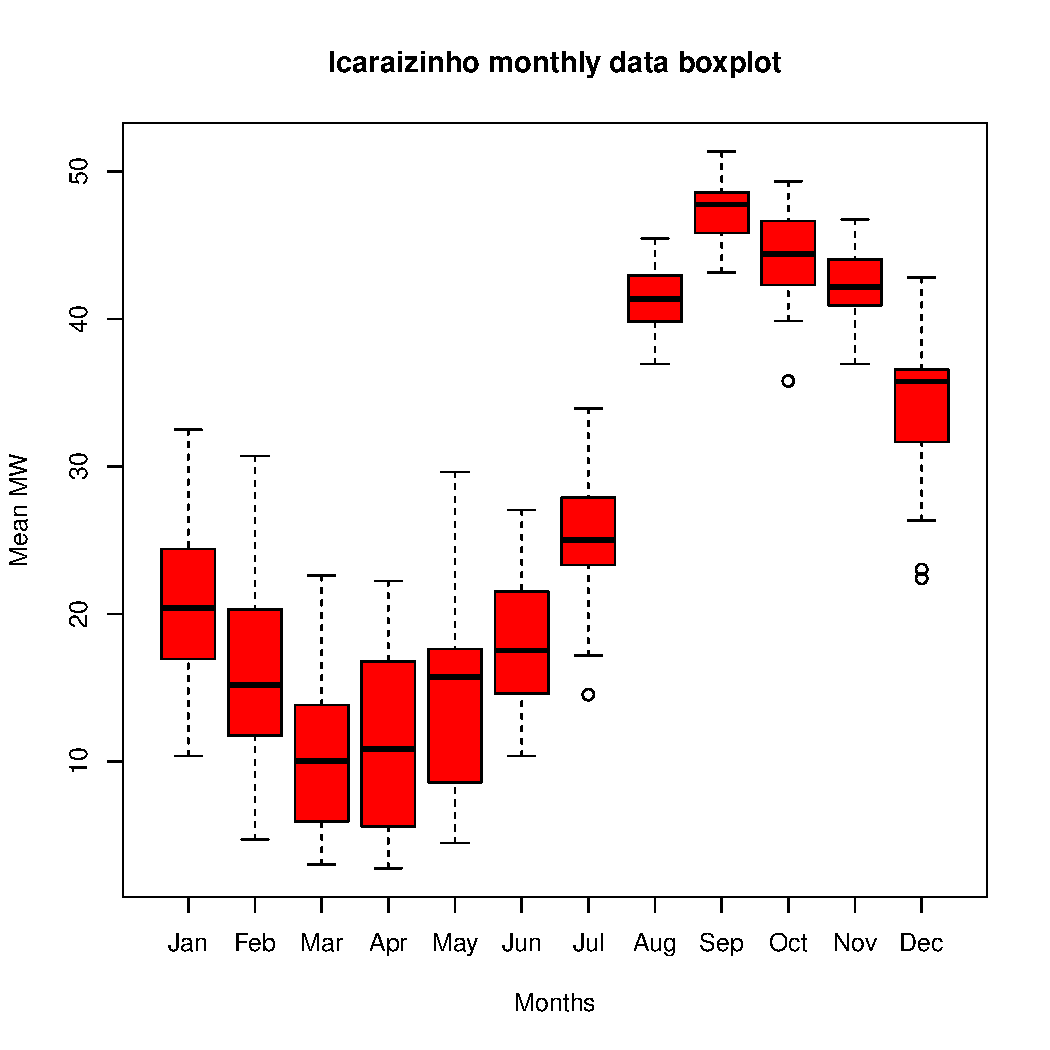
\includegraphics[width=\textwidth]{./../Figuras/Icaraizinho/icaraizinho-boxplot}
%			%\caption{Boxplot for each month for the Icaraizinho dataset}
%			\label{fig:icaraizinho-boxplot}
%		\end{minipage}
%		\begin{minipage}[t]{0.45\linewidth}
%			%\centering
%			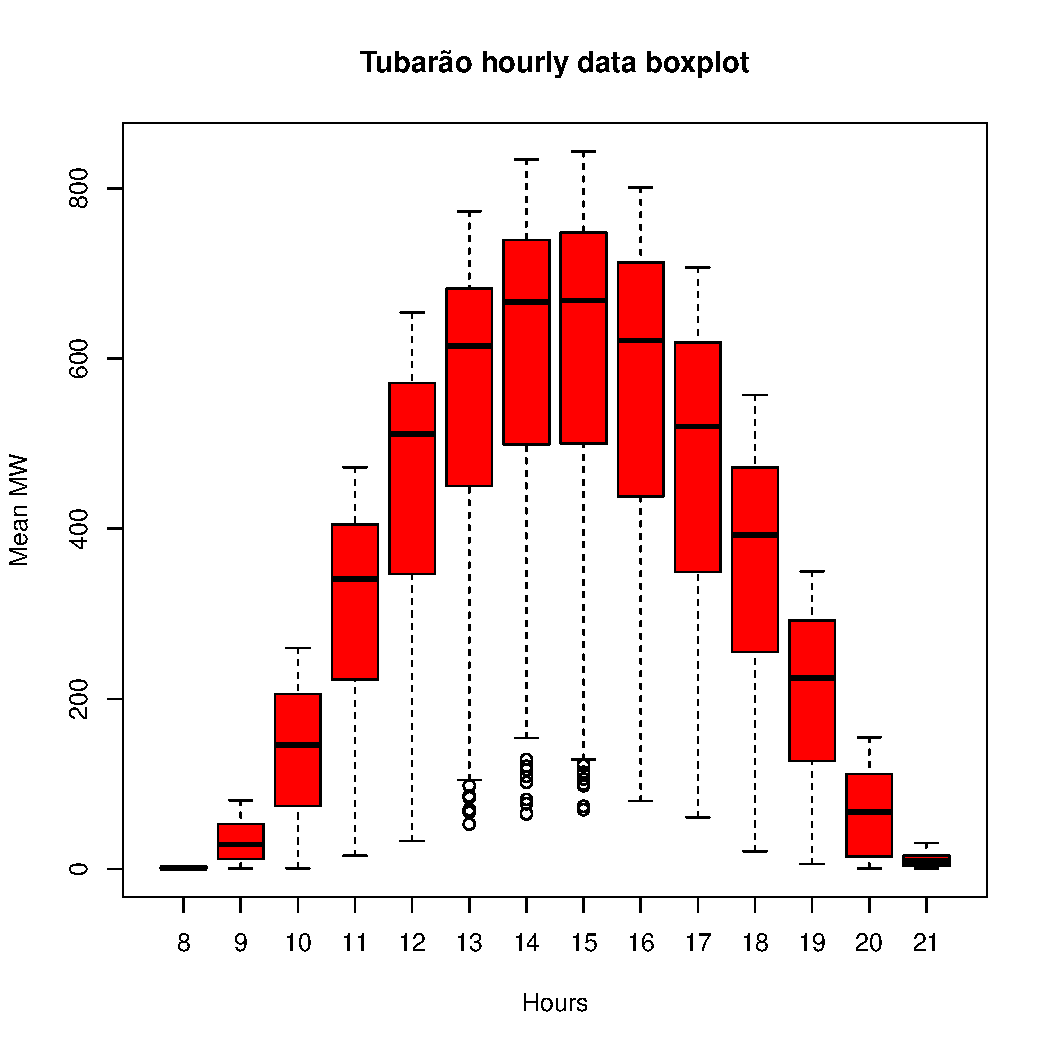
\includegraphics[width=\textwidth]{./../Figuras/Solar-exemplos/tubarao-boxplot}
%			%\caption{Boxplot for each month for the Icaraizinho dataset}
%			\label{fig:tubarao-boxplot}
%		\end{minipage}
%	\end{minipage}
%	\caption{Boxplots showing seasonality for monthly and hourly data.}
%	\label{fig:boxplots}
%\end{figure}


%
%% ===== Sec. III - Regularization ===== %
%
\section{Regularization} \label{sec:regularization}

When dealing with many candidates to use as covariates, one has to deal with the problem of selecting a subset of variables to use in constructing the model. 
This means that the vector of coefficients $\beta_j = [ \beta_{1 j} \cdots \beta_{pj} ]$ should not have all nonzero values.
There are many ways of selecting a subset of variables among the available options.
Classical approaches for this problem are the Stepwise algorithm \cite{efroymson1960multiple}, \cite{hocking_selection_1967}, \cite{tibshirani1996regression}, which includes variables in sequence. 

Two approaches will be employed. At first, we use a Mixed Integer Linear Programming optimization problem (MILP) to find the best subset among all choices of covariates. The second way is by using a LASSO-type technique, which consists in penalizing the $\ell_1$-norm of regressors, thus shrinking the size of estimated coefficients towards zero.  

\subsection{Best subset selection via MILP}
\label{sec:best-subset-mip}

We use MILP to select variables by including constraints which limits their number in $K$. Only $K$ coefficients $\beta_{pj}$ may have nonzero values, for each $\alpha$. 
Binary variable $z_{pj}$ indicates whether $\beta_{pj}$ has a nonzero value. 
The optimization problem that incorporates this idea is described below:
\begin{IEEEeqnarray}{lr}
 \underset{\beta_{0j},\beta_j,z_{p j} \varepsilon_{t j}^{+},\varepsilon_{t j}^{-}}{\text{min}} \sum_{j \in J} \sum_{t\in T}\left(\alpha_j\varepsilon_{t j}^{+}+(1-\alpha_j)\varepsilon_{t j}^{-}\right)  \span \label{eq:mip0}  \\
\mbox{subject to} \span \nonumber \\
\varepsilon_{t j}^{+}-\varepsilon_{t j}^{-}=y_{t}-\beta_{0 j}-\sum_{p=1}^{P}\beta_{p j}x_{t,p}, \span \nonumber  \\
& \forall t \in T ,\forall j \in J, \label{eq:mip1}  \\
\varepsilon_{t j}^{+},\varepsilon_{t j}^{-}\geq0,&\forall t \in T ,\forall j \in J, \label{eq:mip2}\\
- M z_{p j} \leq \beta_{p j} \leq M z_{p j},& \forall j \in J, \forall p\in P, \label{eq:mip3}\\
\sum_{p=1}^P z_{p j} \leq K, &  \forall j \in J, \label{eq:mip4}\\
z_{p j} \in \{0,1\}, & \forall j \in J,  \forall p\in P, \label{eq:mip5}\\
\beta_{0j} + \beta_{j}^T x_{t} \leq \beta_{0,j+1} + \beta_{j+1}^T x_{t},  \nonumber \\
& \forall t \in T, \forall j \in J_{(-1)}, \label{eq:mip6}
\end{IEEEeqnarray}
%\begin{flalign}
%\underset{\beta_{0\alpha},\beta_\alpha,z_{p \alpha}, \varepsilon_{t j}^{+},\varepsilon_{t j}^{-}}{\text{min}} \sum_{j \in J} \sum_{t\in T}\left(\alpha\varepsilon_{t j}^{+}+(1-\alpha)\varepsilon_{tj}^{-}\right) \span \span \label{eq:mip0}   \\
%\mbox{s.t } \nonumber \\
%& \varepsilon_{t j}^{+}-\varepsilon_{t j}^{-}=y_{t}-\beta_{0 \alpha}-\sum_{p=1}^{P}\beta_{p j}x_{t,p}, \span  \label{eq:mip1} \\
%& &  \forall t \in T ,\forall j \in J,  \nonumber\\
%& \varepsilon_{t j}^{+},\varepsilon_{t j}^{-}\geq0, & \forall t \in T ,\forall j \in J, \label{eq:mip2}\\
%& - M z_{p \alpha} \leq \beta_{p j} \leq M z_{p \alpha},& \forall j \in J, \forall p\in P, \label{eq:mip3}\\
%& \sum_{p=1}^P z_{p \alpha} \leq K, & \forall j \in J, \label{eq:mip4}\\
%& z_{p \alpha} \in \{0,1\}, & \forall j \in J,  \forall p\in P, \label{eq:mip5}\\
%& \beta_{0\alpha} + \beta_{\alpha}^T x_{t} \leq \beta_{0\alpha'} + \beta_{\alpha'}^T x_{t}, \span \label{eq:mip6} \\
%& & \forall t \in T, \forall (\alpha, \alpha') \in A \times A,  \alpha < \alpha',   \nonumber
%\end{flalign}
The objective function and constraints (\ref{eq:mip1}), (\ref{eq:mip2}) and (\ref{eq:mip6}) are the same from standard linear quantile regression. 
By constraint (\ref{eq:mip3}), variable $z_{p j}$ is a binary that assumes 1 when coefficient $\beta_{p j}$ is included, while (\ref{eq:mip4}) guarantees that at most $K$ of them are nonzero.
The value of $M$ is chosen in order to guarantee that $M \geq \|\hat{\beta_hj}\|_{\infty}$. The solution given by $\beta_{0j}^*$ and $\beta_j^* = [ \beta_{1 j}^* \cdots \beta_{pj}^* ]$ will be the best linear $\alpha$-quantile regression with $K$ nonzero coefficients.  

\subsubsection{Defining groups for variables}

Consider the optimization problem defined on (\ref{eq:mip0})-(\ref{eq:mip6}). The choice of the best subset is independent for different values of probabilities $\alpha$. This means that the best subset may include two completely different sets of regressors for two probabilities $\alpha_j$ and $\alpha_{j+1}$. Take $K=2$ for the example, selecting $\beta_{1j}$ and $\beta_{4j}$ for $j$ while $\beta_{2,j+1}$ and $\beta_{5,j+1}$ is possible, but unlikely to be true.  

To address this issue, we propose to divide all $j \in J$ in groups. The collection $G$ of all groups $g$ form a partition of $A$, and each $\alpha$ belongs to exactly one group $g$. 
The subset of selected covariates must be the same for all $j$ in the same group $g$. To model these properties as constraints on problem (\ref{eq:mip0})-(\ref{eq:mip6}), we substitute constraint (\ref{eq:mip3}) for the following equations:
\begin{IEEEeqnarray}{lr}
z_{p j g} := 2 - ( 1-z_{pg}) - I_{gj}\span  \label{mipgrupzpa} \\
\sum\limits_{g \in G} I_{gj} = 1, &\forall j \in J,\label{eq:mipgrupa} \\
-Mz_{p j g}  \leq  \beta_{p j} \leq M z_{p j g}, \nonumber \\ 
& \forall p \in P, \forall j \in J,  \forall g \in G,  \label{eq:mipgrupb} \\
I_{gj}, z_{pg} \in \{0,1\}, & \forall p \in P,  \forall g \in G, \label{eq:mipgrupc}
\end{IEEEeqnarray}
%\begin{align} - DUAS COLUNAS
%z_{p \alpha g} := 2 - ( 1-z_{pg}) - I_{g\alpha}\span \span \label{mipgrupzpa} \\
%\sum\limits_{g \in G} I_{g\alpha} = 1, & \forall j \in J,\label{eq:mipgrupa}& \\
%-Mz_{p \alpha g}  \leq  \beta_{p \alpha g} \leq M z_{p \alpha g}, \forall p \in P, \forall j \in J,  \forall g \in G, \span \span \label{eq:mipgrupb} \\
%&I_{g\alpha}, z_{pg} \in \{0,1\},& \, \forall p \in P,  \forall g \in G, \label{eq:mipgrupc}
%\end{align}
on problem (\ref{eq:mip0})-(\ref{eq:mip6}).
where $G$ is a set of group index and $z_{pg}$ is a binary variable that equals 1 iff covariate $p$ is included on group $g$ and $I_{gj}$ equals 1 iff the $j$\textsuperscript{th} quantile belongs to group $g$. 
Constraint (\ref{eq:mipgrupb}) forces that 
$$\text{if }z_{pg} = 0 \text{ and }I_{gj} =1 \text{ then } \beta_{p j = 0}.$$
Hence, if covariate $p$ belongs to group $g$, this covariate is not among group's $g$ subset of variables, than its coefficient must be equal to $0$, for that $j$.
Note that variable $z_{p j}$ behaves differently than when we are not considering groups. This means that if the $j$\textsuperscript{th} quantile belongs to group $g$ but variable $p$ is not selected to be among the ones of group $g$, than $\beta_{pj}$ is zero.
Equation (\ref{mipgrupzpa}) defines $z_{pj}$ to simplify writing. 


%\subsubsection*{Defining groups for variables where each group consists of probabilities in sequence}
%%
%Each groups $g \in G$, as defined on the last section, may be any combination of probabilities $\alpha$, such that they don't be in sequence. Figure \ref{fig:heatmap-exemplo-grupos} shows an example of 
%
%\begin{figure}
%	\centering
%	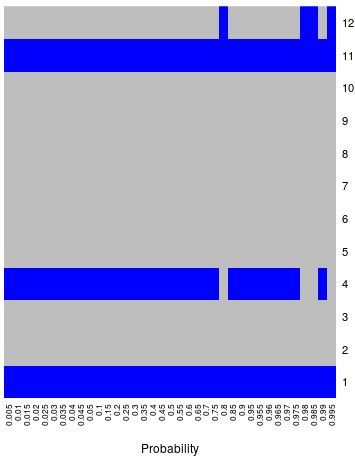
\includegraphics[width=0.4\linewidth]{Figuras/betas-mip/heatmap-exemplo-grupos}
%	\caption{}
%	\label{fig:heatmap-exemplo-grupos}
%\end{figure}
%
%
%\begin{eqnarray}
%\underset{\beta_{0\alpha},\beta_\alpha,z_{p \alpha}, \phi_{p \alpha}, \varepsilon_{t j}^{+},\varepsilon_{t j}^{-}}{\text{min}} & \sum_{j \in J} \sum_{t\in T}\left(\alpha\varepsilon_{t j}^{+}+(1-\alpha)\varepsilon_{tj}^{-}\right) \label{eq:mipgr0} \\
%\mbox{s.t } & \varepsilon_{t j}^{+}-\varepsilon_{t j}^{-}=y_{t}-\beta_{0 \alpha}-\sum_{p=1}^{P}\beta_{p j}x_{t,p},& \qquad\forall t \in T ,\forall j \in J, \label{eq:mipgr1}\\
%& \varepsilon_{t j}^{+},\varepsilon_{t j}^{-}\geq0,&\qquad\forall t \in T ,\forall j \in J, \label{eq:mipgr2}\\
%& - M z_{p \alpha} \leq \beta_{p j} \leq M z_{p \alpha},&\qquad \forall j \in J, \forall p\in\{1,\dots,P\}, \label{eq:mipgr3}\\
%& \sum_{p=1}^P z_{p \alpha} \leq K, & \qquad \forall j \in J, \label{eq:mipgr4}\\
%& z_{p \alpha} \in \{0,1\},&\qquad \forall j \in J, \forall p\in\{1,\dots,P\}, \label{eq:mipgr5}\\
%& \beta_{0\alpha} + \beta_{\alpha}^T x_{t} \leq \beta_{0\alpha'} + \beta_{\alpha'}^T x_{t}, & \qquad \forall t \in T, \forall (\alpha, \alpha') \in A \times A,  \alpha < \alpha',\nonumber\\ \label{eq:mipgr6} \\
%& z_{p\alpha} - z_{p\alpha+1} \leq m_{p\alpha}, & \qquad \forall j \in J', \qquad \forall p \in P  \\
%& \sum_{j \in J'} r_\alpha \leq |G| - 1 
%\label{eq:mipgr} \\
%\end{eqnarray}
%where $A' = A\setminus \{|A|\}$

\subsubsection{Inclusion of derivative penalty}

To incorporate the idea of similarity between coefficients of similar probabilities $\alpha$, we propose to use a penalty on the difference of coefficients. The sequence of coefficients $\{\beta_{pj}\}_{j \in J}$, for a parameter $p$, must have limited second difference, bringing smoothness to the change of coefficients. By including this constraint, every time a variable enters or leaves the subset, its values must be increasing or decreasing smoothly. The second order differential of coefficients is given by the equation below:
\begin{equation}
\tilde{D}_{pj}^{2}:=\frac{\left(\frac{\beta_{p,j+1}-\beta_{pj}}{\alpha_{j+1}-\alpha_{j}}\right)-\left(\frac{\beta_{p,j}-\beta_{p,j-1}}{\alpha_{j}-\alpha_{j-1}}\right)}{\alpha_{j+1}-2\alpha_{j}+\alpha_{j-1}}.
\end{equation}
This idea is implemented on the optimization problem by adding a penalty on the objective function to penalize the absolute value $|D_{pj'}^{2}|$ by a tuning parameter $\gamma$, that controls how rough the sequence $\{\beta_{pj}\}_{j \in J}$ can be. The full optimization problem for the best subset selection via MILP which incorporates the derivative penalty is given below:
\begin{IEEEeqnarray}{lr}
	\underset{\beta_{0j},\beta_j,z_{p j} \varepsilon_{t j}^{+},\varepsilon_{t j}^{-}}{\text{min}} \sum_{j \in J} \sum_{t\in T}\left(\alpha_j\varepsilon_{t j}^{+}+(1-\alpha_j)\varepsilon_{tj}^{-}\right) \nonumber \span \\
	& + \gamma \sum_{j \in J'} D2_{pj}   \\
	\mbox{subject to} \span \nonumber \\
	\varepsilon_{t j}^{+}-\varepsilon_{t j}^{-}=y_{t}-\beta_{0 j}-\beta_{j}^T x_{t,p},& \forall t \in T ,\forall j \in J,\\
	\varepsilon_{t j}^{+},\varepsilon_{t j}^{-}\geq0, & \forall t \in T ,\forall j \in J, \\
	- M z_{p \alpha} \leq \beta_{p j} \leq M z_{p \alpha}, & \forall j \in J, \forall p\in P, \\
	\sum_{p=1}^P z_{p \alpha} \leq K, & \forall j \in J, \\
	z_{p \alpha} \in \{0,1\}, & \forall j \in J,  \forall p\in P, \\
	D2_{pj} >  \tilde D_{pj}^{2} &  \forall j \in J_{(-1)}, \forall p\in P, \\
	D2_{pj} > - \tilde D_{pj}^{2} &  \forall j \in J_{(-1)}, \forall p\in P,\\
\beta_{0j} + \beta_{j}^T x_{t} \leq \beta_{0,j+1} + \beta_{j+1}^T x_{t},&\forall t \in T, \forall j \in J_{(-1)}, 
\end{IEEEeqnarray}
where $A'$ is the set formed by the same elements of $A$ without the first and the last elements.

\subsection{Variable selection via LASSO}
\label{sec:best-subset-ell1}

Another way of doing regularization is including the $\ell_1$-norm of the coefficients on the objective function. In \cite{belloni_l1-penalized_2009}, the reader can find properties and convergence rate when using the LASSO to select variables in a quantile regression setting. The ADALASSO variant is presented in \cite{ciuperca_adaptive_2016}. 
The advantage of this method is that coefficients are shrunk towards zero by changing a continuous parameter $\lambda$, which penalizes the size of the $\ell_1$-norm.  
When the value of $\lambda$ gets bigger, fewer variables are selected to be used. 
This is the same strategy of the LASSO methodology, and its usage for the quantile regression is discussed in \cite{li2012l1}.
On the litterature, the LASSO QR regularization is applied for only a single quantile by the following optimization problem:
\begin{equation}
\underset{\beta_{0\alpha},\beta_\alpha}{\text{min}} \sum_{t \in T}\alpha|y_{t}-q_\alpha(x_t)|^{+}+ \sum_{t \in T}(1-\alpha)|y_{t}-q_\alpha(x_t)|^{-}+\lambda\|\beta_\alpha\|_{1},
\label{eq:l1-qar-optim}
\end{equation}
\[
q_\alpha(x_t)=\beta_{0}-\sum_{p=1}^{P}\beta_{p}x_{t,p}.
\]
In our problem, however, we need to estimate multiple quantiles in a way that the issue of crossing quantiles is circumvented. So, we use for the LASSO the same formulation of estimating all quantiles simultaneously with a non crossing constraint relating each quantile function.



The process of estimation is done in two stages: variable selection and coefficients estimation. At first, all normalized covariates\footnote{For such estimation to be coherent each covariate must have the same relative weight in comparison with one another, i.e., they must be normalized. 
This normalization process is a linear transformation to each covariate such that all have mean $\mu = 0$ and variance $\sigma^2 = 1$. 
We apply the transformation $\tilde{x}_{t,p} = (x_{t,p} - \bar{x}_{t,p}) / \hat\sigma_{x_{t,p}}$, where $\bar{x}_{t,p}$ and $\hat{\sigma}_{x_{t,p}}$ are respectively the sample's unconditional mean and standard deviation. The $\tilde{y}_{t-p,i}$ series will be used to estimate the coefficients, as this series has the desired properties.} are input on the following optimization problem:
\begin{IEEEeqnarray}{lr}
\tilde \beta_\lambda^{*LASSO} = \underset{\beta_{0},\beta,\varepsilon_{t j}^{+},\varepsilon_{t j}^{-}}{\text{arg min}} \sum_{j \in J} \sum_{t \in T}(\alpha_j\varepsilon_{t j}^{+}+(1-\alpha_j)\varepsilon_{t j}^{-}) \span \nonumber \\
\hspace{3.5cm} +\lambda\sum_{p=1}^{P}\mbox{\ensuremath{\xi}}_{p j} + \gamma \sum_{j \in J'} D2_{pj} \span \label{eq:obj-lasso} \\
\mbox{subject to } \nonumber & \\
\varepsilon_{t j}^{+}-\varepsilon_{t j}^{-}=y_{t}-\beta_{0 j}-\beta_{j}^T x_{t,p},& \forall t \in T ,\forall j \in J,\\\varepsilon_{t j}^{+},\varepsilon_{t j}^{-}\geq0,&\forall t \in T, \forall j \in J,\\
\xi_{pj}\geq\beta_{p j},&\forall p\in P, \forall j \in J,  \label{l1-qar-3}
\\
\xi_{pj}\geq - \beta_{p j},&\forall p\in P, \forall j \in J,  \label{l1-qar-4}
\\
	D2_{pj} >  \tilde D_{pj}^{2} &  \forall j \in J_{(-1)}, \forall p\in P, \\
D2_{pj} > - \tilde D_{pj}^{2} &  \forall j \in J_{(-1)}, \forall p\in P,\\
\beta_{0j} + \beta_{j}^T x_{t} \leq \beta_{0,j+1} + \beta_{j+1}^T x_{t},&\forall t \in T, \forall j \in J_{(-1)}, \label{eq:l1-qar5}
\end{IEEEeqnarray}
This model is built upon the standard linear programming model for the quantile regression (\ref{eq:linear-opt-1})-(\ref{eq:linear-opt-ult}). 
On the above formulation, the $\ell_1$ norm of equation (\ref{eq:l1-qar-optim}) is substituted by the sum of $\xi_p$, which represents the absolute value of $\beta_{pj}$. The link between variables $\xi_p$ and $\beta_{pj}$ is made by constraints (\ref{l1-qar-3}) and (\ref{l1-qar-4}). Note that the linear coefficient $\beta_{0j}$ is not included in the penalization, as the sum of penalties on the objective function \ref{eq:obj-lasso}.

% % % % % % % % Esse trecho deve ser usado quando os coeficientes do lasso forem utilizados, e não apenas o lasso sendo um seletor de variáveis % % % % % % % % %
%Each component of the output $\tilde \beta_\lambda^{*LASSO}$ must be corrected by multiplying each coefficient for its standard deviation: $\beta_{p\alpha,\lambda}^{*LASSO} = \tilde \beta_{p\alpha,\lambda}^{*LASSO} \hat\sigma_{x_{t,p}}$.
%\begin{eqnarray}
%\tilde \beta_\lambda^{*LASSO} = \underset{\beta_{0},\beta,\varepsilon_{t j}^{+},\varepsilon_{t j}^{-}}{\text{arg min}} & \sum_{j \in J} \sum_{t \in T}\left(\alpha\varepsilon_{t j}^{+}+(1-\alpha)\varepsilon_{t j}^{-}\right)+\lambda\sum_{p=1}^{P}\mbox{\ensuremath{\xi}}_{p \alpha} \label{eq:obj-lasso} \\
%\mbox{subject to } & \varepsilon_{t j}^{+}-\varepsilon_{t j}^{-}= y_{t}-\beta_{0 \alpha}-\sum_{p=1}^{P}\beta_{p j}\tilde x_{t,p},&\forall t\in T, \forall j \in J, \\
%& \varepsilon_{t j}^{+},\varepsilon_{t j}^{-}\geq0,&\forall t \in T, \forall j \in J,\\
%& \xi_{pj}\geq\beta_{p j},&\forall p\in P, \forall j \in J,  \label{l1-qar-3}
%\\
%& \xi_{pj}\geq-\beta_{p j},&\forall p\in P, \forall j \in J.  \label{l1-qar-4}
%\end{eqnarray}

For low values of $\lambda$, the penalty over the size of coefficients is small. Because of that, the output of problem (\ref{eq:obj-lasso})-(\ref{l1-qar-4}) is a model where most coefficients have nonzero value. On the other hand, when the penalty on $\| \beta_j \|_1$ is big, many covariates will have zero valued coefficients. When $\lambda$ approaches infinity, one has a constant model. 
For instance, the penalty isn't applied to the linear coefficient $\beta_{0j}$. 

In fact, the LASSO coefficients are biased, so it is employed only as a variable selector. 
The optimum vector of coefficients $\tilde \beta_\lambda^{*LASSO}$ for a given $\lambda$ may be composed by both nonzero and zero coefficients. 
We then define $S_\lambda$ as the set of indexes of selected variables given by
\begin{equation*}
S_\lambda = \{ p \in \{ 1,\dots,P \} | \; |\beta^{*LASSO}_{\lambda,p}| \neq 0  \}.
\end{equation*}
Hence, we have that, for each $p \in \{ 1,\dots,P \}$,
$$\beta^{*LASSO}_{\lambda,p} = 0 \Longrightarrow \beta^{*}_{\lambda,p} = 0.$$

Note that problem (\ref{eq:linear-opt-1})-(\ref{eq:linear-opt-ult}) is employed to act as variable selection only. On the second stage, the optimal coefficient vector $\beta_\lambda^{*LASSO}$ is estimated by the non-regularized QR, where only variables that bellongs to $S_\lambda$ are input:
\begin{IEEEeqnarray*}{lr} (\mathcal{L}_{\lambda}^{*},\beta_{\lambda}^{*})\overset{(obj,var)}{\longleftarrow} \underset{\beta_{0j},\beta_j,z_{p j}, \varepsilon_{t j}^{+},\varepsilon_{t j}^{-}}{\text{min}} \sum_{j \in J} \sum_{t\in T}\left(\alpha_j \varepsilon_{t j}^{+}+(1-\alpha_j)\varepsilon_{t\alpha_j}^{-}\right) \span \nonumber
\\
&  + \gamma \sum_{j \in J'} D2_{pj} \\
\text{subject to } \span \nonumber \\
\varepsilon_{t j}^{+}-\varepsilon_{t j}^{-}=y_{t} - \beta_{0\alpha} - \sum_{p\in S_\lambda} \beta_p x_{t,p}, & \forall t \in T, \forall j \in J, \\
\varepsilon_{tj}^+,\varepsilon_{tj}^- \geq 0, &  \forall t \in T,\forall j \in J,\\ 
D2_{pj} >  \tilde D_{pj}^{2} &  \forall j \in J_{(-1)}, \forall p\in P, \\
D2_{pj} >  - \tilde D_{pj}^{2} &  \forall j \in J_{(-1)}, \forall p\in P,\\
\beta_{0j} + \beta_{j}^T x_{t} \leq \beta_{0,j+1} + \beta_{j+1}^T x_{t}, & \forall t \in T, \forall j \in J_{(-1)},
\end{IEEEeqnarray*}
The variable $\mathcal{L}_{\lambda}^{*}$ receives the value of the objective function on its optimal solution.
In summary, the optimization in equation \ref{eq:l1-qar-optim} acts as a variable selection for the subsequent estimation, which is normally called the post-LASSO estimation \cite{belloni2009least}.



% (\ref{eq:linear-opt-1})-(\ref{eq:linear-opt-ult}). 




%


%% ===== Sec. IV - Simulation ===== %

\section{Simulation}
\label{sec:simulation}

In this section, we investigate how to simulate future paths of the time series $y_t$. 
%We use this model to produce $K$ future values for the time serie $y_t$. 
Let $n$ be the total number of observations of $y_t$. We produce $S$ different paths with size $K$ for each. 
We have $n$ observations of $y_t$ and a vector of explanatory variables $x_t$.
The variables chosen to compose $x_t$ can be either exogenous variables, autoregressive components of $y_t$ or both. We use a nonparametric approach which to estimate, at every $t$, the $k$-step ahead conditional density of $y_t$.

To produce $S$ different paths of $\{ \hat{y}_t \}_{t=n+1}^{n+K}$, we use the following procedure:

\noindent\rule{\columnwidth}{3pt}

Procedure for simulating $S$ scenarios of $y_t$

\noindent\rule{\columnwidth}{1pt}

\begin{enumerate}
	
\item At first, let $\tau = n + 1$.

\item In any given period $\tau$, for every $\alpha \in A$, we use one of the methods presented in the last sections to estimate the value of each $\alpha$-quantile.
Note that $x_{\tau}$ is supposed to be known at time $\tau$. In the presence of exogenous variables that are unknown, it is advisable to incorporate its uncertainty by considering different scenarios. In each scenario, though, $x_{\tau}$ must be considered fully known. 
 
\item Let $\hat{Q}_{y_{\tau}|X}(\alpha,x_\tau)$ be the estimated quantile function of ${y}_{\tau}$. 
To estimate $\hat{Q}_{y_{\tau}}$, we first define a discrete quantile function $\tilde{Q}_{y_\tau}$. By mapping every $\alpha \in A$ with its estimated quantile $\hat{q}_{\alpha}$, we define function $\tilde{Q}_{y_{\tau}}$. When we interpolate 

%This process is described in more details on section \ref{sec:estimating-distribution}. 

\item Once we have a distribution for $y_{n+1}$, we can generate $S$ different simulated values, drawn from the distribution function $\hat{F}_{y_{n+1}} = \hat{Q}^{-1}_{y_{\tau}}$, derived from the quantile function found by doing steps 2 and 3. 
Let $X$ be a random variable with uniform distribution over the interval $[0,1]$. By using results from the Probability Integral Transform, we know that the random variable $F^{-1}_{y_{n+1}}(X)$ has the same distribution as $y_{n+1}$. So, by drawing a sample of size $S$ from $X$ and applying the quantile function $Q_{y_{n+1}}(\alpha)$, we have our sample of size $K$ for $y_{n+1}$.

\item Each one of the $S$ different values for $y_{n+1}$ will be the starting point of a different path. Now, for each $\tau \in [n+2,n+K]$ and $s \in S$, we have to estimate quantiles $q_{\alpha \tau, s}$ and find a quantile function for $\hat{Q}_{y_{\tau,s}}$ just like it was done on steps 2 and 3.
Note that when $\tau > n+2$, every estimate will be scenario dependent, hence there will be $S$ distribution functions estimated for each period $\tau$. From now on, in each path just one new value will be drawn randomly from the one-step ahead distribution function - as opposed to what was carried on step 3, when $S$ values were simulated. As there will be $S$ distribution functions - one for each path, in each period $\tau$ it will be produced exact $S$ values for $y_\tau$, one for its own path. Repeating this step until all values of $\tau$ and $s$ are simulated will give us the full simulations that we are looking for.
\end{enumerate}

\noindent\rule{\columnwidth}{1pt}

%\noindent\rule{\textwidth}{1pt}

%\subsection{Simulating for a seasonal time series}

%Construir seção

%% ===== Sec. V - Estimation ===== %
%
\section{Estimation}

\subsection{Time-series cross validation}

Sections \ref{sec:best-subset-mip} and \ref{sec:best-subset-ell1} presented two different methods to estimate the conditional distribution in a parsimonious way. However, as presented, the aforementioned methods don't provide a unique solution, but a set of solutions for a range of tuning parameters. For instance, on the MILP method, the quantity $K$ of nonzero coefficients is an input of the problem. Similarly, the LASSO needs a penalization parameter $\lambda$, that tunes how much penalty the $\ell_1$-norm receives.

In statistics and machine learning, a popular technique is using Cross-validation (CV) to select the best model from this range of possibilities.
It is a technique used to have an estimative of the model's quality of prediction in an independent testing set. The best model that minimizes the CV error is the model which presumably will have the best performance on out of sample data.

The usage of CV is not straightforward when data is dependent, which is the case when working with time series. As the data is time dependent, one can be interested in using either all observations or to take the dependency away. The works
\cite{bergmeir_note_2017} and \cite{bergmeir_use_2012} deals specifically with the usage of CV in a time series context. They provide tests with both $K$-fold CV and $K$-fold with non-dependent data. Both schemes are shown of Figure \ref{fig:cross-validation-scheme}.
This mimics real applications better even by dropping in a few times the number of observations. Will use a growing window in a 5-fold scheme.
\begin{figure}
	\centering
	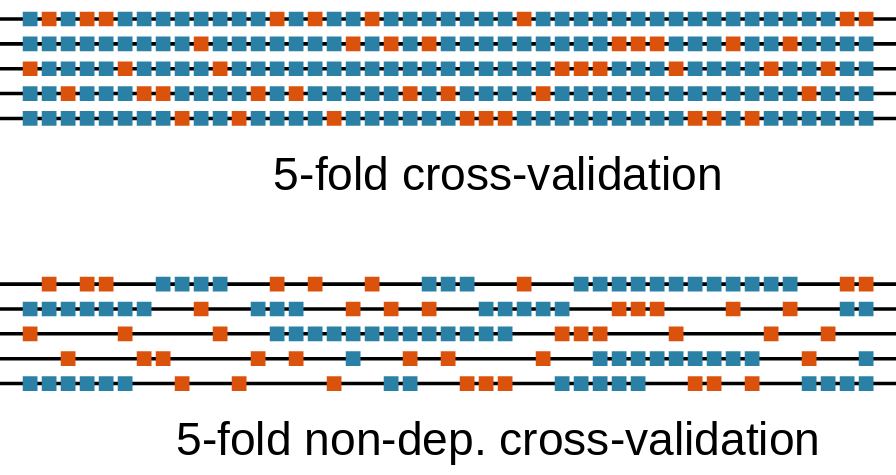
\includegraphics[width=0.9\linewidth]{Figuras/Cross-validation-scheme}
	\caption{$K$-fold CV and $K$-fold with non-dependent data. Observations in blue are used to estimation and in orange for evaluation. Note that non-dependent data doesn't use all dataset in each fold.}
	\label{fig:cross-validation-scheme}
\end{figure}
In both settings, the training data is randomly split into a collection of sets $J_k$, forming a $K$ size partition. Each of these $J_k$ is used as test set, while \todoi{terminar parágrafo de explicação sobre CV}

% \todoi{Ver se novas figuras (R/grafico-cv.r) e ver se incluir outras formas de CV} % escolhemos trabalhar apenas com este tipo de CV



\subsection{Information Criteria for Quantile Regression}
Sometimes, using CV can be computationally expensive, as the full estimation is done several times for each tuning parameter - in this case, either $K$ or $\lambda$. Other form of deciding the quantity of variables that provides a good equilibrium between in-sample prediction and parsimony is the Information Criteria.

Information criteria summarizes two aspects. One of them refers to how well the model fits the in-sample observations and the other part penalizes the quantity of covariates used in the model. By penalizing how big our model is, we prevent overfitting from happening. So, in order for a covariate to be included in the model, it must supply enough goodness of fit.
In \cite{machado1993robust}, it is presented a variation of the Schwarz criteria for M-estimators that includes quantile regression. The Schwarz Information Criteria (SIC), adapted to the quantile autoregression case, is presented below:
\begin{align} 
\begin{split}
SIC(m) = n \log({obj}^*)+\frac{1}{2}K\log n,\label{eq:SIC}
\end{split}					
\end{align}
where $K$ is the model's dimension. This procedure leads to a consistent model selection if the model is well specified. 

By minimizing the $SIC$ \todoi{acabar}

\subsection{Model selection distance}
%
%On sections \ref{sec:best-subset-mip} and \ref{sec:best-subset-ell1}, we presented two ways of selecting variables. Nonetheless, regularization can be done with different levels of parsimony. For example, one can select a different number $K$ of variables to be included in the best subset selection via MILP or choose different values of $\lambda$ for the $\ell_1$ penalty. 
%There is a tradeoff between variability and bias, when selecting the number of variables in a model. In order to  

% % % Métrica

Solving a LP problem such as the LASSO is many times faster than a similar-sized MILP problem, for introducing binary variables breaks the problem's convexity. On the other hand, in our case the MILP solution is the exact best solution in minimizing the QR objective function, while the LASSO is an approximation of that.

One of our goals is to test how far from the optimal solution is the LASSO.
%It would be interesting, then, to use a faster method that would provide a solution close to the optimal. 
%To test how far are the solutions given by both methods, we propose an experiment that is described as follows. 
For each number $K$ of total nonzero coefficients, there will be a penalty $\lambda^*_K$ which minimizes the errors from the quantile regression's objective function (given on equation (\ref{eq:post-lasso})): 
%\todo{($K$ ranging from 0 until 12, where 0 means that only the intercept is included)}
\begin{equation}
\lambda^*_K = \argmin_\lambda \left\lbrace \left.  obj_{\lambda}^{*} \quad  \right| \, \| \beta^*_\lambda \|_0 = K \right\rbrace,
\end{equation}
where the quantity $\| \beta^*_\lambda \|_0$ is the $0$-norm, which gives the total of nonzero coefficients, for a given lambda of the LASSO estimations.

We, then, define the sets $L_K^{LASSO}$ and $L_K^{MILP}$, which contains all nonzero indexes, for a given $K$, when using methods LASSO and MILP for regularization, respectively.
Thus, we can compare the best LASSO fit where exactly $K$ variables are selected with the best fit given by the MILP problem, also with $K$ variables selected.

As the MILP solution is the exact solution for the problem, while the LASSO solution is an approximation, we use the former as a \textit{benchmarking} for the quality of the latter solution. It is desirable that the LASSO solution be as related with the MILP solution as possible. The difference in performance is given by a similarity metric $d$, which measures distance from solutions weighted by the correlation between variables. 
The similarity is calculated as the solution of the following optimization problem
\begin{IEEEeqnarray}{lC}
	d(\beta^*_{MILP(K)}, \beta^*_{\lambda^*_K}) = \min_{0\leq\delta_{ij}\leq1} & \sum\limits_{i,j = 1}^K  \delta_{ij} (1-|\rho_{ij}|) \label{eq:metricad0} \\
	\text{subject to} & \nonumber \\
	\sum\limits_{j =1}^K\delta_{ij}=1, &  i=1,\dots,K,\\
	\sum\limits_{i =1}^K\delta_{ij}=1, & j=1,\dots,K,
\end{IEEEeqnarray}
where $\rho_{ij}$ is the correlation between the $i$-th and $j$-th independent variables in sets $L_k^{MILP}$ and $L_k^{LASSO}$, respectively. The optimal value for the decision variables of this problem provides us with an assignment between selected covariates from both methods, namely, MILP and LASSO, that minimizes the overall ``index of uncorrelation" between selected covariates. If $\delta^*_{ij} = 1$, the $i$-th selected variable in  $L_k^{MILP}$ is associated with the $j$-th variable  in $L_k^{LASSO}$. For instance, if $d(\beta^*_{MILP(K)}, \beta^*_{\lambda^*_K}) = 0$, it means that there are $K$ perfectly correlated pair of variables, even though not being the same subset. 


\subsection{Evaluation criteria}
The full dataset is split between the test set - which evaluates our methodology's forecasting performance - and the training set - which we use to estimate parameters.  This setting mimics real world applications, where the future is unknown.

As conditional distribution is the focus in this paper, we use a performance measurement which emphasizes the correctness of each quantile. 
For each observation $y_t$ and probability $\alpha \in A$, a score function
is defined by

\[
L(A)= \sum_{t\in T}\rho_{\alpha}(y_{t}-q_{\alpha}(x_t))
\]
The error measure is defined as the average of the score function
for all observations and target quantiles.


% % % Trocar o sigma da função objetivo.




% % % recolocar no texto







\bibliographystyle{IEEEtran}
\bibliography{Thesis,QR,Bibhenriquinho}



\end{document}
